\section{Capitolo 4}

	\subsection{Esercizio 4.1}
Scrivere una function Matlab che implementi il calcolo del polinomio interpolante di grado $n$ in forma di Lagrange. La forma della function deve essere del tipo \texttt{ y = lagrange( xi, fi, x ) }.

La base di Lagrange è così definita:
\begin{equation}
	L_{kn} := \prod_{j=0,j\neq{k}}^n\frac{x-x_j}{x_k-x_j}
\end{equation}
La forma di Lagrange del polinomio interpolante è:
\begin{equation}\label{lagrange_equation}
	\sum_{k=0}^n f(x_k) L_{kn}(x)
\end{equation}
La function Matlab che implementa la \ref{lagrange_equation} è:
\lstinputlisting{./capitolo_4/lagrange.m}


	\subsection {Esercizio 4.2}
Scrivere una function Matlab che implementi il calcolo del polinomio interpolante di grado $n$ in forma di Newton. La forma della function deve essere del tipo \texttt{ y = newton( xi, fi, x ) }

La base di Newton è così definita: 
\begin{empheq}[left=\empheqlbrace]{align}
	& \omega_0(x):=1 \\
	& \omega_1(x):=x-x_0 \\
	& ... \\
	& \omega_{i+1}(x):=(x-x_i)\omega_i(x)
\end{empheq}
La forma di Newton del polinomio interpolante rispetto alla base di Newton è:
\begin{equation} \label{newton_equation}
	\sum_{k=0}^n f[x_0, ... , x_k]\omega_k(x)
\end{equation} 
La function matlab che implementa \ref{newton_equation} è:
\lstinputlisting{./capitolo_4/newton.m}

	\subsection {Esercizio 4.3}
Scrivere una function Matlab che implementi il calcolo del polinomio interpolante di Hermite. La forma della function deve essere del tipo \texttt{ y = hermite( xi, fi, f1i, x ) }

Il polinomio interpolante di Hermite richiede un numero pari di ascisse distribuite come segue: 
\begin{equation}
	a <= x_0 < x_{\frac{1}{2}} < x_{1+\frac{1}{2}} < ... < x_n < x_{n+\frac{1}{2}} <= b
\end{equation}
con $\lim{x_{i+\frac{1}{2}} = x_i}$ si ha che $x_0 = x_1$, $x_2=x_3$, etc. Pertanto $f[x_i, x_1]:=f[x_i, x_i]:=f^{(1)}(x_i)$ e l'algoritmo delle differenze divise verrà modificato in modo che al primo passo quando bisogna calcolare $f[x_i, x_i]$ si utilizza il valore della derivata prima che verrà passato come parametro alla funzione.

La function Matlab che implementa il polinomio interpolante di Hermite è:
\lstinputlisting{./capitolo_4/hermite.m}

	\subsection {Esercizio 4.4}
Utilizzare le functions degli esercizi precedenti per disegnare l'approssimazione della funzione $sin(x)$  nell'intervallo $[0, 2\pi]$, utilizzando le ascisse di interpolazione $x_{i}=i\pi, i=0,1,2$.

Il codice seguente richiama le funzioni definite in precedenza e disegna un grafico con il confronto fra le funzioni $sin(x)$ e i corrispondenti polinomi interpolanti in forma di Newton e di Lagrange.
\lstinputlisting{./capitolo_4/sin_interpolation.m}
Il risultato è stato riportato in figura \ref{sin_interpolation}. \textbf{ verificare perché bisogna usare ascisse $0\pi, 1\pi, 2\pi$ }.

\begin{figure}\label{sin_interpolation}
    \centering
    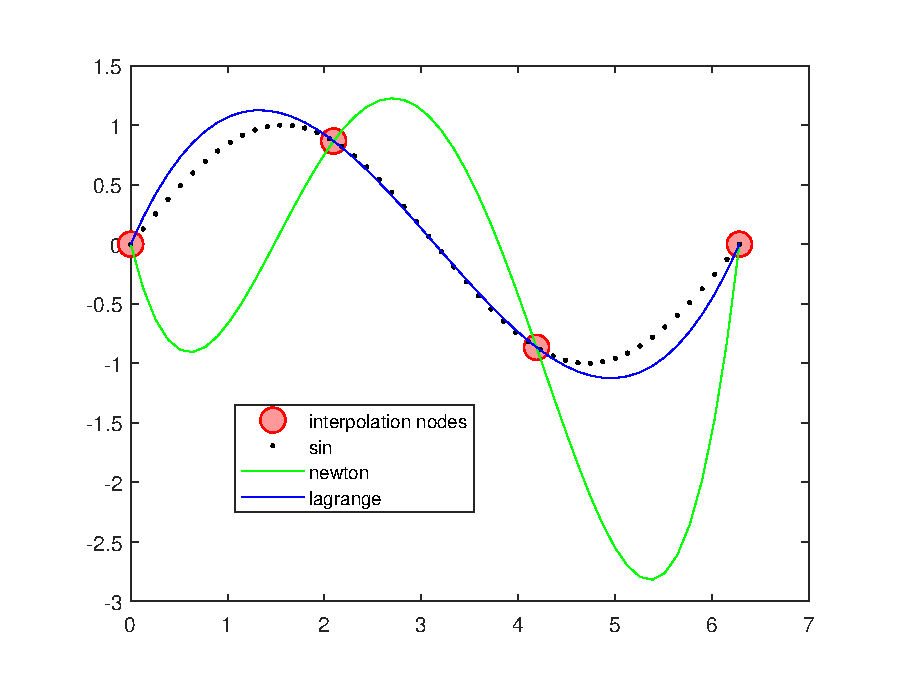
\includegraphics{./capitolo_4/sin_interpolation}
    \caption{Interpolazione usando forma di Lagrange e di Newton}
\end{figure} 

	\subsection {Esercizio 4.5}
Scrivere una function Matlab che implementi la \texttt { spline } cubica interpolante (naturale o \textit{not-a-knot}, come specificato in ingresso) delle coppie di dati assegnate. La forma della function deve essere del tipo: \texttt { y = spline3( xi, fi, x, tipo ) }.

Formula per il calcolo della spline cubica:
\begin{equation}
	s_3(x) = \frac{(x - x_{i-1})^2m_i + (x_i-x)^2m_{i-1}}{6h_i} + q_i, \;\; x \in [x_{i-1}, x_i]
\end{equation}

Condizioni per il calcolo della spline naturale:
\[
	\begin{pmatrix}
		2 		& \epsilon_1 	& 			& 		& 	\\
		\phi_2 	& 2			& \epsilon_2	& 		& 	\\
				& ...			& ...			& ... 	& 	\\
				& 			& ...			& ... 	& \epsilon_{n-2}	\\
				& 			& 			& \phi_{n-1} 	& 2	\\
	\end{pmatrix}
	\begin{pmatrix}
		m_1 \\
		m_2 \\
		... \\
		... \\
		m_{n-1}
	\end{pmatrix}
	= 6
	\begin{pmatrix}
		f[x_0, x_1, x_2] \\
		m_2 \\
		... \\
		... \\
		m_{n-1}
	\end{pmatrix}
\]
Condizioni per il calcolo della spline cubica:

	\subsection {Esercizio 4.6}
Scrivere una function Matlab che implementi il calcolo delle ascisse di Chebyshev per il polinomio interpolante di grado $n$, su un generico intervallo $[a,b]$. La function deve essere del tipo: \texttt { xi = ceby( n, a, b ) }.

	\subsection {Esercizio 4.7}
Utilizzare le function degli Esercizi 4.1 e 4.6 per graficare l'approssimazione della funzione di Runge sull'intervallo $[-6,6]$ per $n= 2,4, ... ,40$. Stimare, numericamente, l'errore commesso in funzione del grado $n$ del polinomio interpolante.

	\subsection {Esercizio 4.8}
Relativamente al precedente esercizio, stimare numericamente, la crescita della costante di Lebesgue.

	\subsection {Esercizio 4.9}
Utilizzare la function dell'esercizio 4.1 per approssimare la funzione di Runge sull'intervallo $[-6,6]$, su una partizione uniforme di $n+1$ ascisse, $n= 2,4, ... ,40$. Stimare le corrispondenti costanti di Lebesgue.

	\subsection {Esercizio 4.10}
Stimare, nel senso dei minimi quadrati, posizione, velocità iniziale ed accelerazione relative a un moto rettilineao uniformemente accelerato per cui sono note le seguenti misurazioni delle coppie (tempo, spazio): (1, 2.9), (1, 3.1), (2, 6.9), (2, 7.1), (3, 12.9), (3, 13.1), (4, 20.9), (4, 21.1), (5, 30.9), (5, 31.1).